\documentclass[UTF8,12pt]{ctexart}
\usepackage{amsmath,amssymb,geometry,bm,graphicx,fontspec,amssymb,amsthm}
\usepackage[mathscr]{euscript}

\usepackage[colorlinks,
linkcolor=black,
anchorcolor=blue,
citecolor=green
]{hyperref} % 目录中的超链接

\newtheorem{Def}{定义}[section]
\newtheorem{Theo}{定理}[section]
\newtheorem{Lemm}{引理}[section]
\newtheorem{Prop}{命题}[section]
\newtheorem{Assu}{假设}[section]
\newtheorem{Axiom}{Axiom}

\numberwithin{equation}{section} % 按章节进行排序与编号
\numberwithin{figure}{section}
\numberwithin{table}{section}

\usepackage{draftwatermark} % 所有页加水印
\SetWatermarkText{EconNerd} % 设置水印内容
\SetWatermarkLightness{0.99} % 设置水印透明度 0-1
\SetWatermarkScale{1} % 设置水印大小    

\title{审计} % 文档相关信息
\author{EconNerd}
\date{\today}
\geometry{scale=0.8}

\begin{document}
	\maketitle
	\tableofcontents
	\newpage

	\section{审计概述}
	\subsection{审计的概念与保证程度}
	\paragraph{审计的分类}审计的概念有很大,不同种类的审计有着不同的定义。审计分类可以分为政府审计与注册会计师审计。或者内审与外审。分类上不同的审计有着不同的特征。
	
	\paragraph{CPA的业务以及审计和审阅的区分}注册会计师的业务主要可以分为鉴证业务和相关服务。
	\begin{enumerate}
		\item 鉴证业务
		\begin{enumerate}
			\item 审计(例如,财务报表审
			计、企业内部控制审计等),提供合理保证。通常以积极方式提出结论
			
			\item 审阅,提供有限保证,主要以询问和分析程序为主。通常以消极方式提出结论
			
			\item 其他鉴证业务(例如,预
			测性财务信息审核),提供合理保证或有限保证
			(不可一概而论)
		\end{enumerate}
		
		\item 相关服务,以下业务不提供任何程度的保证。
		\begin{enumerate}
			\item 代编财务信息
			
			\item 对财务信息执行商定程序
			
			\item 税务咨询
			
			\item 管理咨询
		\end{enumerate}
	\end{enumerate}
	
	\paragraph{财务报表审计的含义}财务报表审计是指注册会计师对财务报表是否不存在重大错报提供合理保证,以积极方式提出意见,增强除管理层之外的预期使用者对财务报表信赖的程度。
	
	用户为财务报表的预期使用者。目的为(1)改善财务报表的质量,增强管理层之外的预期使用者对财务报表的
	信赖程度,即以合理保证的方式提高财务报表的可信度;
	(2)不涉及为如何利用信息提供建议。
	
	在\textbf{保证程度}上(1)由于固有限制,审计提供的是合理保证,而非绝对保证;(2)大多数审计证据是说服性而非结论性的。
	
	审计的基础为(1)注册会计师的独立性:独立于被审计单位和预期使用者;(2)注册会计师的专业性,最终产出的产品为审计报告。
	
	\paragraph{职业责任、期望差距和信息差距}
	\begin{enumerate}
		\item 职业职责。指注册会计师作为一个职业对社会公众应尽的责任,在很大程度上反映相关方(特别是财务报表使用者)的期望。
		
		\item 期望差距。社会公众与注册会计师职业界在对职业责任的认识上存在的差距导致期望差距,注册会计师应充分关注舞弊风险,了解并尽可能缩小期望差距。
		
		\item 信息差距。短式标准审计报告存在着信息含量低、相关性差等缺陷,而现行审计报告,特别是引进关键审计事项部分,提高了审计报告的相关性和决策有用性,缩小了信息差距。
	\end{enumerate}
	
	
	\subsection{审计要素}
	审计要素主要包括五个部分:审计业务的三方关系人、财务报表、财务报告编制基础、审计证据、审计报告
	
	\paragraph{审计业务的三方关系人}
	三方人包括
	\begin{enumerate}
		\item 注册会计师。遵守相关职业道德要求,按照审计准则的规定对财务报表发表审计意见是注册会计师的责任。
		
		\item 被审计单位的管理层。执行\textbf{审计工作的前提}(注意和审计的前提条件进行区分)是管理层管理层和治理层认可并理解其应当承担的下列三项责任:
		\begin{enumerate}
			\item 编制之责:按适用的财务报告编制基础编制财务报表,并使其实现公允反映;
			
			\item 内控之责:设计、执行和维护必要的内部控制,以使财务报表不存在由于舞弊或错误
			导致的重大错报;
			
			\item 条件之责:向注册会计师提供必要的工作条件,包括:
			a.允许注册会计师接触与编制财务报表相关的所有信息;
			b.向注册会计师提供审计所需的其他信息;
			c.允许注册会计师在获取审计证据时不受限制地接触其认为必要的内部人员和其他相关人员。
		\end{enumerate}
		
		管理层或治理层对编制财务报表承担\textbf{完全责任},财务报表审计并不减轻管理层或治理层的责任。
		
		如果财务报表存在重大错报,而注册会计师通过审计没有发现,并不能因此减轻管理层和治理层对财务报表的责任。
		
		\item 预期使用者。范围上包含主要利益相关者,通常包括股东、公司债权人、证券监管机构等
	\end{enumerate}
	
	预期使用者与注册会计师的关系
	(1)注册会计师可能无法识别使用审计报告的所有组织和人员;
	(2)审计报告的收件人应当尽可能明确为所有的预期使用者
	
	预期使用者与管理层的关系
	(1)注册会计师的审计意见主要是向除管理层之外的预期使用者提
	供的;
	(2)管理层可能是预期使用者,但不能是唯一预期使用者;
	(3)管理
	\paragraph{财务报表}
	(1)在财务报表审计中,审计对象是历史的财务状况、经营成果(财务业绩)和现金流量。
	(2)审计对象信息(即审计对象的载体)是财务报表(包括相关附注)。
	
	\paragraph{财务报告编制基础}
	(1)在财务报表审计中,财务报告编制基础即是标准。财务报告编制基础分为通用目的编制基础和特殊目的编制基础。
	(2)注册会计师基于自身的预期、判断和个人经验对鉴证对象进行的评价和计量,不构成适当的标准。
	(3)对于公开发布的标准,注册会计师通常无须对标准的适当性进行评价,只需评价
	该标准对具体业务的适用性。
	
	\paragraph{审计证据}
	审计证据主要是在审计过程中通过\textbf{实施审计程序获取},包括:
	\begin{enumerate}
		\item 内部来源的信息,如会计记录等;
		
		\item 外部来源的信息,如专家编制的信息等;
		
		\item 以前审计中获取的信息;
		
		\item 接受与保持客户或业务时实施质量管理程序获取的信息。
	\end{enumerate}
	
	审计证据的特点上。
	(1)既包括支持和佐证管理层认定的信息,也包括与这些认定相矛盾的信息;
	(2)某些情况下,信息的缺乏(如管理层拒绝提供要求的书面声明)本身也构成审计
	证据。
	
	\paragraph{审计报告}
	注册会计师应当针对财务报表在所有重大方面是否符合适当的财务报告编制基础,以书面报告的形式发表能够提供合理保证程度的意见。
	
	\subsection{审计目标}
	审计目标分为两个层次,总体审计目标和具体审计目标
	
	\paragraph{财务报表审计的总体目标}
	总体审计目标主要关注于两个方面
	\begin{enumerate}
		\item \textbf{发表审计意见}。对财务报表整体是否不存在由于舞弊或错误导致的重大错报获取合理保证,使注册会计师能够对财务报表是否在所有重大方面按照适用的财务报告编制基础编制发表审计意见
		
		\item \textbf{出具审计报告}。按照审计准则的规定,根据审计结果对财务报表出具审计报告,并与管理层和治理层沟通
	\end{enumerate}
	
	2.审计准则的要求对实现总体目标的作用
	(1)注册会计师恰当执行审计准则的要求,预期能为其实现目标提供充分的基础。
	(2)由于各项审计业务的具体情况存在很大差异,并且审计准则不可能预想到所有的
	情况,注册会计师有责任确定必要的审计程序,以满足审计准则的要求和实现目标。
	(3)针对某项业务的具体情况,可能存在一些特定事项,需要注册会计师实施审计准
	则要求之外的审计程序,以实现审计准则规定的目标。
	
	\paragraph{认定和具体审计目标}
	
	认定与具体审计目标密切相关,注册会计师的基本职责就是确定被审计单位管理层对\textbf{财务报表的认定是否恰当(即是否存在重大错报)}。注册会计师了解认定,才能相对应地确定每个项目的具体审计目标。
	
	认定是指管理层针对财务报表要素的确认、计量和列报(包括披露)作出一系列明确或暗含的意思表达。对于管理层对财务报表各组成要素作出的认定,注册会计师的审计工作就
	是要确定管理层的认定是否恰当。
	
	我们主要关注资产负债表和利润表的认定
	\begin{enumerate}
		\item 所审计期间各类交易事项及相关披露的认定(利润表)
		\begin{enumerate}
			\item 发生。已发生,且与被审计单位有关。真实发生、并非虚构
			
			\item 完整性。已记录,相关披露均已包括。没有遗漏、没有隐瞒
			
			\item 准确性。有关的金额已恰当记录,相关披露已得到恰当计量和描述。计算参数和运算过程准确无误
			
			\item 截止。已记录于正确的会计期间。没有提前、没有推迟。
			
			\item 分类。已记录于恰当的账户。没有表内串户
			
			\item 列报。已被恰当地汇总或分解且表述清楚,相关披露是相关的、可理解的。
		\end{enumerate}
		
		\item 期末账户余额及相关披露的认定(资产负债表)
		\begin{enumerate}
			\item 存在。记录的资产、负债和所有者权益是存在的。真实存在,并非虚构
			
			\item 权利和义务。记录的资产由被审计单位拥有或控制;记录的负债是被审计单位应履行的偿还义务。对已记录的资产和负债享有权利、承担义务
			
			\item 完整性。已记录,相关披露均已包括。没有遗漏、没有隐瞒
			
			\item 准确性、计价和分摊。以恰当金额包括在财务报表中,相关的计价或分摊调整已恰当记录,相关披露已得到恰当计量和描述。期末余额以及折摊、减值准确无误
			
			\item 分类。已记录于恰当的账户。没有表内串户
			
			\item 列报。已被恰当地汇总或分解且表述清楚,相关披露是相关的、可理解的。
		\end{enumerate}
	\end{enumerate}
	
	权利和义务以及存在之间需要区分一下。且值得注意的是,完整性的违反特征是未记录,截止的违反特征是提前或推迟记录,其他的违反特征都是已记录为前提。
	
	\subsection{审计基本要求}
	审计的基本要求包含四个:1.遵守审计准则2.遵守职业道德守则3.保持职业怀疑4.运用职业判断
	
	\paragraph{遵守审计准则}
	
	审计准则是衡量注册会计师执行财务报表审计业务的权威性标准,涵盖从接受业务委托到出具审计报告的整个过程,注册会计师在执业过程中应当遵守审计准则的要求。
	
	\paragraph{遵守职业道德守则}
	
	注册会计师职业道德守则基本原则包括六个方面,即诚信、独立性、客观公正、专业胜任能力和勤勉尽责、保密以及良好职业行为。
	
	\paragraph{保持职业怀疑}

	职业怀疑指注册会计师执行审计业务的一种态度,包括采取质疑的思维方式,对可能表明由于舞弊或错误导致错报的情况保持警觉,以及对审计证据进行审慎评价。主要要求如下
	\begin{enumerate}
		\item 秉持质疑的理念。职业怀疑与职业道德基本原则的关系是:
		①职业怀疑与职业道德基本原则相互关联。
		②保持独立性可以增强注册会计师在审计中保持客观公正、职业怀疑的能力。
		
		\item 对引起疑虑的情形保持警觉。应当运用职业怀疑的情形包括但不限于:
		①相互矛盾的审计证据;
		②引起对文件记录、对询问答复的可靠性产生怀疑的信息;
		③表明可能存在舞弊的情况;
		④表明需要实施除审计准则规定外的其他审计程序的情形。
		
		\item 审慎评价审计证据。
		①质疑相互矛盾的审计证据的可靠性;
		②注册会计师可以在审计成本与信息的可靠性之间进行权衡,但审计中的困难、时间或成
		本等事项本身,不能作为省略不可替代的审计程序或满足于说服力不足的审计证据的理由。
		
		\item 客观评价管理层和治理层。
		不应依赖以往对管理层和治理层诚信形成的判断。即使认为管理层和治理层是正直、诚
		实的,也不能降低保持职业怀疑的要求,不允许在获取合理保证的过程中满足于说服力不足
		的审计证据。
	\end{enumerate}
	
	保持职业怀疑是保证审计质量的关键要素,有助于注册会计师恰当运用职业判断,提高审计程序设计及执行有效性,降低检查风险,对发现舞弊、防止审计失败至关重要。
	
	影响职业怀疑的事项和因素。
	(1)会计师事务所的业绩评价、薪酬和晋升机制会促进或削弱审计实务中对职业怀疑的保持程度,这取决于这些机制如何设计和执行。
	(2)会计师事务所人员是否能够保持职业怀疑,很大程度上取决于其胜任能力。
	
	\paragraph{运用职业判断}
	1.含义
	(1)在审计准则、财务报告编制基础和职业道德要求的框架下,综合运用相关知识、技能和经验,作出适合审计业务具体情况、有根据的行动决策。
	(2)职业判断是注册会计师行业的精髓,职业判断能力是注册会计师胜任能力的核心。
	(3)如果有关决策不被该业务的具体事实和情况所支持,或者缺乏充分、适当的审计
	证据,职业判断并不能作为注册会计师不恰当决策的理由。
	
	职业判断运用环节包括从决定是否接受业务委托,到出具业务报告的各类决策:
	(1)与具体会计处理相关的决策;
	(2)与审计程序相关的决策;
	(3)与遵守职业道德守则要求相关的决策
	
	具体情形包括
	\begin{enumerate}
		\item 确定重要性,识别和评估重大错报风险;

		\item 确定所需实施的审计程序的性质、时间安排和范围;

		\item 评价证据是否充分、适当,是否需要执行更多的工作;

		\item 评价管理层在运用适用的财务报告编制基础时作出的判断;

		\item 根据已获取的审计证据得出结论,如评估管理层在编制财务报表时作出的会计估计的合理性;

		\item 运用职业道德概念框架识别、评估和应对对职业道德基本原则产生的不利影响
	\end{enumerate}
	
	提高职业判断质量的方式
	(1)丰富的知识、经验和良好的专业技能;
	(2)独立、客观和公正;
	(3)保持职业怀疑。
	
	衡量职业判断质量的标准主要包括五条。
	\begin{enumerate}
		\item 准确性或意见一致性。
		准确性:
		职业判断结论与特定标准或客观事实的相符程度
		
		意见一致性:
		不同职业判断主体针对同一职业判断问题所作判断彼此认同的程度
		
		\item 决策一贯性和稳定性。
		决策一贯性:
		同一注册会计师针对同一项目的不同判断问题,所作出的判断之间是否符合应有的内在逻辑
		
		稳定性:
		同一注册会计师针对相同的职业判断问题,在不同时点所作出的判断是否结论相同或相似
		
		\item 可辩护性。是否能够证明自己的工作。可辩护性的基础通常包括:
		①理由的充分性;
		②思维的逻辑性;
		③程序的合规性
	\end{enumerate}

	\subsection{审计风险}
	审计风险主要有两类:\textbf{重大错报风险以及检查风险}。
	\paragraph{重大错报风险}
	指财务报表在审计前存在重大错报的可能性。重大错报风险与被审计单位的风险相关,且独立于财务报表审计而存在,属于\textbf{客观存在的风险}。
	
	重大错报风险包含\textbf{财务报表层次和认定层次两个层次},注册会计师应当从两个层次考虑重大错报风险。
	
	\textbf{财务报表层次的重大错报风险}指与财务报表整体存在广泛联系的重大错报风险。①通常与控制环境和其他因素(如经济萧条)有关;
	②增加了认定层次发生重大错报的可能性;
	③需要考虑舞弊引起的特别风险;
	④难以界定于某类具体认定,通常影响多项不同的认定
	
	\textbf{认定层次的重大错报风险}
	指与某类交易、事项,期末账户余额或财务报表披露相关的重大错报风险。认定层次的重大错报风险\textbf{可以进一步细分为固有风险和控制风险}。认定层次的重大错报风险=固有风险×控制风险
	
	\textbf{固有风险}是指在不考虑控制的情况下,某一认定易于发生错报的可能性
	
	固有风险因素可以是定性的,也可以是定量的,包括:
	①事项或情况的复杂性、主观性、变化、不确定性;
	②管理层偏向;
	③其他舞弊风险因素;
	④产生经营风险的外部因素
	
	\textbf{控制风险}是指某一认定发生错报,该错报单独或连同其他错报是重大的,但没有被内部控制及时防止或发现并纠正的可能性
	
	
	对固有风险和控制风险的评估要求
	(1)财务报表层次:对于识别出的财务报表层次重大错报风险,审计准则未明确规定,是应当分别评估固有风险和控制风险,还是合并评估。注册会计师识别和评估财务报表层次重大错报风险采用的具体方法,\textbf{取决于其偏好的审计技术方法以及实务上的考虑}。
	(2)认定层次:对于识别出的认定层次重大错报风险,注册会计师\textbf{应当分别评估}固有风险和控制风险。
	
	\paragraph{检查风险}
	检查风险指如果存在某一错报,该错报单独或连同其他错报可能是重大的,注册会计师为将审计风险降至可接受的低水平而实施程序后没有发现这种错报的风险。
	
	
	(1)检查风险取决于审计程序设计的合理性和执行的有效性;
	(2)由于注册会计师通常并不对所有交易、账户余额和披露进行检查,以及其他原因,不可能将检查风险降低为零。
	
	降低检查风险的途径
	(1)适当计划审计工作;
	(2)在项目组成员之间进行恰当的职责分配;
	(3)保持职业怀疑的态度;
	(4)监督、指导和复核项目组成员执行的审计工作。
	
	\paragraph{审计风险模型——重大错报风险与检查风险的关系}
	
	审计风险指当财务报表存在重大错报时,注册会计师发表不恰当审计意见的可能性。审计风险取决于重大错报风险和检查风险,可以用公式表达为:
	审计风险=重大错报风险×检查风险
	
	“一定两反”原则
	(1)前提:审计风险是既定的。
	(2)两者关系:可接受的检查风险水平与评估的认定层次重大错报风险呈反向关系;
	评估的重大错报风险越高,可接受的检查风险越低。
	
	
	实务中,注册会计师不一定用绝对数量表达这些风险水平,可选用“高”“中”“低”等文字进行定性描述。
	
	\paragraph{审计固有限制}
	许多财务报表项目涉及主观决策、评估或不确定性,例如其金额本身存在一定的变动幅度,这种变动幅度不能通过实施审计程序予以消除。
	
	审计程序的性质
	(1)管理层或其他人员可能有意或无意地不提供与财务报表编制相关的或注册会计师
	要求的全部信息;
	(2)舞弊可能涉及精心策划和蓄意实施以进行隐瞒,注册会计师不应被期望成为鉴定
	文件真伪的专家;
	(3)审计不是对涉嫌违法行为的官方调查。
	
	
	注册会计师在合理时间内以合理成本对财务报表形成审计意见。
	
	\newpage
	\section{审计计划}
	\subsection{初步业务活动}
	审计基本流程通常其实与初步业务活动,终止于出具审计报告。这一过程形成了如下所示的审计地图
	\begin{enumerate}
		\item 初步业务活动
		
		\item 审计计划
		
		\item 风险评估
		
		\item 风险应对
		
		\item 完成审计工作
		
		\item 出具审计报告
	\end{enumerate}
	审计计划、风险评估和风险应对是动态循环过程,在审计过程中不断调整、贯穿始终
	
	\paragraph{初步业务活动的目的和内容}
	\begin{enumerate}
		\item 考量对方。(1)针对保持客户关系和具体审计
		业务实施相应的质量管理程序目的是确定不存在因管理层诚信问题而可能影响注册会计师保持该项业务意愿的事项
		
		\item 打量自身。(2)评价遵守相关职业道德规范要
		求的情况(2)确保具备执行业务所需要的独
		立性和专业胜任能力
		
		\item 达成一致。(3)就审计业务约定条款达成一致
		意见,确保与被审计单位之间不存在对业务约定条款的误解
	\end{enumerate}
	
	\paragraph{审计前提条件}
	包含两条,需要同时满足
	\begin{enumerate}
		\item 审计单位管理层在编制财务报表时采用可接受的财务报告编制基础
		
		\item 管理层对注册会计师执行审计工作的前提的认可(详见第一章)
	\end{enumerate}
	
	具体展开第一条,确定财务报告编制基础的可接受性时的考虑因素包括:
	(1)被审计单位的性质;
	(2)财务报表的目的(包括通用目的编制基础和特殊目的编制基础);
	(3)财务报表的性质;
	(4)法律法规是否规定了适用的财务报告编制基础。
	
	注意区分\textbf{审计前提}和\textbf{执行审计工作}的前提
	\paragraph{审计业务约定书的基本内容和特殊考虑}

	会计师事务所承接任何审计业务,都应与被审计单位签订审计业务约定书。审计业务约定书应当包括以下主要内容:
	\begin{enumerate}
		\item 财务报表审计的目标与范围;
		
		\item 注册会计师的责任;
		
		\item 管理层的责任;
		
		\item 适用的财务报告编制基础;
		
		\item 审计报告的预期形式和内容,以及对在特定情况下出具的审计报告可能不同于预期形式和内容的说明。
	\end{enumerate}
	
	
	
	对于\textbf{组成部分的审计},如果母公司的注册会计师同时也是组成部分注册会计师,需要决定是否向组成部分单独致送审计业务约定书。
	
	对于\textbf{连续审计},注册会计师应当根据具体情况评估是否需要对审计业务约定条款作出修改,以及是否需要提醒被审计单位注意现有的条款;注册会计师可以决定不在每期都致送新的审计业务约定书或其他书面协议。
	
	\paragraph{审计业务变更的影响}
	审计业务变更为保证程度较低的业务的合理性。如果因为
	(1)环境变化对审计服务的需求产生影响
	(2)对原来要求的审计业务的性质存在误解\textbf{则通常合理}。
	
	如果因为\textbf{管理层施加的或其他情况}引起的审计范围受到限制,则\textbf{不一定合理}
	
	
	没有合理的理由,注册会计师不应同意变更业务。如果注册会计师不同意变更审计业务约定条款,而管理层又不允许继续执行原审计业务,注册会计师应当执行以下措施:
	(1)在适用的法律法规允许的情况下,解除审计业务约定;
	(2)确定是否有约定义务或其他义务向治理层、所有者或监管机构等报告该事项。
	
	3.审计业务变更为审阅业务或相关服务的要求
	情形
	
	审计转为审阅或其他相关服务都不应在报告中提及原审计业务和已执行程序。如果转为商定程序则可以提及
	\subsection{总体审计策略和具体审计计划}
	\paragraph{总体审计策略}
	总体审计策略包括四个方面:
	\begin{enumerate}
		\item 确定审计范围,
		
		\item 计划报告目标、时间安排及所需沟通的性质,
		
		\item 确定审计方向,
		
		\item 规划和调配审计资源。
	\end{enumerate}
	
	其中,确定审计方向主要考虑以下几个因素
	\begin{enumerate}
		\item 重要性方向
		
		\item 重大错报风险较高的审计领域
		
		\item 项目组人员的选择和工作分工,包括想重大错报风险较高的审计领域分派具备适当经验的人员
		
		\item 项目预算,包括考虑为重大错报风险可能较高的审计领域分配适当的工作时间等
	\end{enumerate}
	
	
	
	
	\paragraph{具体审计计划}
	\begin{figure}[th]
		\centering
		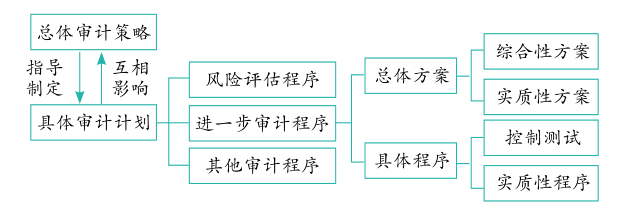
\includegraphics[width=0.7\linewidth]{screenshot001}
		\caption{}
		\label{fig:screenshot001}
	\end{figure}
	
	具体审计计划针对审计程序,其中其他审计程序的内容是考虑特殊事项的审计程序。
	
	\paragraph{审计过程中对计划的更改}
	计划审计工作贯穿于整个审计业务的始终,注册会计师应在必要时对总体审计策略和具体审计计划作出更新和修改。
	
	\paragraph{指导、监督与复核}
	注册会计师应当制定计划,确定对项目组成员的指导、监督以及对其工作进行复核的性
	质、时间安排和范围,主要取决于下列因素:
	(1)被审计单位的规模和复杂程度;
	(2)审计领域;
	(3)评估的重大错报风险;
	(4)执行审计工作的项目组成员的专业素质和胜任能力。
	
	\subsection{重要性}
	
	\subsubsection{重要性的概念}
	重要性的本质是用来衡量错报是否重大。在制定总体审计策略时需要确定重要性。
	
	重要性的判断维度主要是从定量以及定性两个方面进行判断。在定量层面,如果错报金额超过财务报表整体的重要性,则错报通常是重大的。
	
	在定性层面,如果某些错报金额低于财报整体的重要性,并不说明错报不重大。某些错报金额高于财报整体的重要性,但是相对资产负债表占比较小,且对关键信息的披露不产生重大影响,则可能认定这样的错报不重大。
	
	
	重要性的概念包括以下系列:
	\begin{enumerate}
		\item 财务报表整体的重要性;
		
		\item 实际执行的重要性;
		
		\item 特定类别的交易、账户余额或披露的重要性;
		
		\item 明显微小错报的临界值
	\end{enumerate}

	
	在计划和执行审计工作,评价识别出的错报对审计的影响,以及未更正错报对财务报表和审计意见的影响\textbf{以上三个程序}时,注册会计师需要运用重要性概念。
	
	其中计划与执行审计工作可以具体分为风险评估程序与进一步审计程序。进一步审计程序又包括了控制测试与实质性程序(分为细节测试和实质性分析程序)
	
	注册会计师在计划审计工作时对何种情形构成重大错报作出的判断,也同时为下列方面提供了基础:
	\begin{enumerate}
		\item 确定风险评估程序的性质、时间安排和范围;
	
		\item 识别和评估重大错报风险;
	
		\item 确定进一步审计程序的性质、时间安排和范围
		
	\end{enumerate}
	
	\subsubsection{重要性的确定}
	\paragraph{财务报表整体重要性}
	如果合理预期错报单独或连同其他错报可能影响财务报表使用者的决策,则该项错报是重大的。注册会计师通过执行审计工作对财务报表发表审计意见,因此应当考虑财务报表整体的重要性。
	
	
	财务报表整体重要性确定的原则:注册会计师需要运用职业判断确定重要性,经常根据事务所惯例和自身经验予以考虑,但不考虑与具体项目相关的固有不确定性。
	
	具体方法为选定一个“基准”,再乘以某一“百分比”作为财务报表整体的重要性,使用公式可以将其表示为:财务报表整体的重要性=基准×百分比
	
	选择基准的考虑因素。包括:
	\begin{enumerate}
		\item 财务报表要素;
		
		\item 是否存在财务报表使用者特别关注的项目;
		
		\item 被审计单位的性质、所处的生命周期阶段以及所处行业和经济环境;
		
		\item 被审计单位的所有权结构和融资方式;
		
		\item 基准的相对波动性。
	\end{enumerate}
	
	选择基准的示例如下
	\begin{enumerate}
		\item 企业的盈利水平保持稳定。\textbf{经常性业务的税前利润}
		
		
		\item 企业近年来经营状况大幅度波动,盈利和亏损交替发生,或由正常盈利变为微利或微亏,或本年度税前利润因情况变化而出现意外增加或减少
		
		\textbf{过去3~5年经常性业务的平均税前利润或亏损(取绝对值),或其他基准,例如营业收入}
		
		\item 国际企业集团设立的研发中心,主要为集团下属企业提供研发服务,并以成本加成方式向相关企业收取费用。\textbf{成本与营业费用总额}
		
		\item 企业为新设企业,处于开办期,尚未开始经营,目前正在建造厂房及购买机器设备。\textbf{总资产}
		
		\item 企业处于新兴行业,目前侧重于抢占市场份额、扩大知名度和影响力。\textbf{营业收入}
		
		\item 开放式基金,致力于优化投资组合、提高基金净值、为基金持有人创造投资价值。\textbf{净资产}
		
	\end{enumerate}
	
	
	(5)百分比的确定方法(实务中通常为1\%~5\%)。考虑因素包括:
	\begin{enumerate}
		\item 是否为上市公司或公众利益实体;
		
		\item 财务报表使用者的范围;
		
		\item 被审计单位是否由集团内部关联方提供融资或是否有大额对外融资;
		
		\item 财务报表使用者是否对基准数据特别敏感等。
		
	\end{enumerate}
	
	\paragraph{特定类别的交易、账户余额或披露的重要性水平}
	1.含义
	特定类别的交易、账户余额或披露发生错报时,即使错报金额低于财务报表整体的重要性,但如果能够合理预期该错报可能影响报表使用者依据财务报表作出的经济决策,应确定该认定的重要性水平。
	
	确定该重要性的方法主要如下
	\begin{enumerate}
		\item 法律法规或适用的财务报告编制基础是否影响财务报表使用者对特定项目计量或披露的预期关联方交易、管理层和治理层的薪酬等
		
		\item 与被审计单位所处行业相关的关键性披露制药企业的研究与开发成本等
		
		\item 财务报表使用者是否特别关注财务报表中单独披露的业务的特定方面重大企业合并的披露等
	\end{enumerate}
	
	
	实务操作上主要有两种情况
	(1)特定类别交易、账户余额或披露的重要性水平应低于财务报表整体的重要性;
	(2)与财务报表整体的重要性相同,认定层次的重要性也需要相应确定实际执行的重要性。
	
	\paragraph{实际执行的重要性}
	
	实际执行的重要性,是指注册会计师确定的低于财务报表整体重要性的一个或多个金额,旨在将未更正和未发现错报的汇总数超过财务报表整体重要性的可能性降至适当的低水平;如果适用,还指注册会计师确定的低于特定类别的交易、账户余额或披露的重要性水平的一个或多个金额。
	
	在确定该重要性时主要考虑如下几个因素
	\begin{enumerate}
		\item 对被审计单位的了解;
		
		\item 前期审计工作中识别出的错报的性质和范围;
		
		\item 根据前期识别出的错报对本期错报作出的预期。
	\end{enumerate}
	
	实务操作上通常财务报表层次实际执行的重要性通常为财务报表整体重要性的50\%~75\%。根据不同情形进行变化。
	
	3.实务运用
	(1)注册会计师在计划审计工作时可以根据实际执行的重要性确定需要对哪些类型的
	交易、账户余额和披露实施进一步审计程序,即通常选取金额超过实际执行的重要性的财务
	报表项目。
	(2)不代表注册会计师可以对所有金额低于实际执行的重要性的财务报表项目不实施
	进一步审计程序,这是由于:
	①单个金额低于实际执行的重要性的财务报表项目汇总起来可能金额重大,注册会计师
	需要考虑汇总后的潜在错报风险;
	②对于存在低估风险的财务报表项目,不能仅仅因为其金额低于实际执行的重要性而不
	实施进一步审计程序;
	③对于识别出存在舞弊风险的财务报表项目,不能因为其金额低于实际执行的重要性而
	不实施进一步审计程序。
	
	\paragraph{明显微小错报的临界值}
	1.含义
	(1)如果注册会计师将低于某一金额的错报界定为明显微小的错报,这些错报无论从
	规模、性质或其发生的环境,无论单独或者汇总起来,都是明显微不足道的。
	(2)注册会计师应当在审计工作底稿中记录设定的明显微小错报临界值,低于该金额
	的错报视为明显微小的错报,可以不累积。
	(3)“明显微小”不等同于“不重大”。
	(4)如果不确定一个或多个错报是否明显微小,就不能认为这些错报是明显微小。
	2.确定方法
	(1)经验百分比:通常为财务报表整体重要性的3%至5%,通常不超过10%,除非注册
	会计师认为有必要单独为重分类错报确定一个更高的临界值。
	(2)考虑因素:
	①以前年度审计中识别出的错报(包括已更正和未更正错报)的数量和金额;
	②重大错报风险的评估结果;
	③被审计单位治理层和管理层对注册会计师与其沟通错报的期望;
	④被审计单位的财务指标是否勉强达到监管机构的要求或投资者的期望。
	
	\subsubsection{审计过程中修改重要性}
	由于下列原因,注册会计师可能需要修改财务报表整体的重要性和特定类别的交易、账
	户余额或披露的重要性水平:
	(1)审计过程中情况发生重大变化(如决定处置被审计单位的一个重要组成部分);
	(2)获取新信息;
	(3)通过实施进一步审计程序,注册会计师对被审计单位及其经营所了解的情况发生
	变化。
	
	\subsubsection{错报}
	1.概念
	错报指某一财务报表项目的金额、分类或列报,与按适用的财务报告编制基础应列示的
	金额、分类、列报之间存在的差异;以及根据注册会计师的判断,为使财务报表在所有重大
	方面实现公允反映,需要对金额、分类、列报作出必要的调整。
	2.来源
	错报来源于舞弊或错误。
	3.类型
	事实错报
	定义
	收集或处理数据错误,对事实的误解或忽略,或故意舞弊行为。
	本质是违反客观事实
	示例
	存货、固定资产的入账价值录入错误,与发票、合同等不符
	判断错报
	定义
	(1)管理层和注册会计师对会计估计值的判断差异;
	(2)管理层和注册会计师对选择和运用会计政策的判断差异
	示例
	投资性房地产公允价值不合理;存货发出采用后进先出法核算
	推断错报
	定义
	通常指根据样本推断的总体错报
	示例
	运用审计抽样,通过测试样本估计出的总体的错报减去在测试中
	发现的已经识别的具体错报
	4.识别和更正
	(1)错报可能不会孤立发生,一项错报的发生还可能表明存在其他错报。
	(2)抽样风险和非抽样风险可能导致某些错报未被发现(相关概念在“审计抽样方
	法”章节详解)。审计过程中累积错报的汇总数接近确定的重要性,表明存在比可接受的低
	风险水平更大的风险,即可能未被发现的错报连同审计过程中累积错报的汇总数,可能超过
	重要性。
	(3)通常,注册会计师应当及时将审计过程中累积的所有错报与适当层级的管理层进
	行沟通,还应当要求管理层更正这些错报。
	
	
	\newpage
	\section{审计证据}	
	\subsection{审计证据的性质}
	审计证据是指注册会计师为了得出审计结论、形成审计意见而使用的所有信息。
	
	审计证据的所有信息是与审计过程相对应的概念。包括在\textbf{初步业务活动、审计测试流程、完成审计工作与出具审计报告}这几个过程中获得的审计证据。
	
	审计证据主要考虑两个性质,充分性与适当性。一个代表量一个代表质。质可以影响量,反之不行。适当性中,只有相关且可靠的审计证据才是高质量的。
	
	评价审计证据时还有以下几个特殊考虑
	\begin{enumerate}
		\item 对文件记录可靠性的考虑
		
		\item 使用被审计单位生成信息时的考虑
		
		\item 证据相互矛盾时的考虑
		
		\item 获取审计证据时对成本的考虑
	\end{enumerate}
	
	\subsection{审计程序}
	基本的审计程序包括了\textbf{检查、观察、询问、函证、重新计算、重新执行和分析}。这些基本的审计程序组合起来也可以形成其他的审计程序。
	
	在审计测试流程过程中,不同的阶段(程序)会使用不同的审计程序。
	\begin{enumerate}
		\item 风险评估程序:检查、观察、询问、分析程序
		
		\item 控制测试(进一步审计程序):检查、观察、询问、重新执行
		
		\item 实质性程序(进一步审计程序):细节测试使用检查、观察、询问、函证、重新计算
		
		\item 实质性程序(进一步审计程序):实质性分析程序使用分析程序
	\end{enumerate}
	
	\subsection{函证}
	函证相关的内容主要考虑如下的因素
	\begin{enumerate}
		\item 函证决策
		
		\item 函证设计
		
		\item 函证发出
		
		\item 函证收回与否,以及函证过程中设计的舞弊风险迹象的应对措施
	\end{enumerate}
	
	\subsubsection{函证决策}
	函证决策的考虑因素可以分为应当考虑和可以考虑两类,应当考虑的因素如下
	\begin{enumerate}
		\item 评估的认定层次重大错报风险
		
		\item 函证程序针对的认定
		
		\item 实施除函证以外其他的审计程序
	\end{enumerate}
	
	可以考虑的因素如下
	\begin{enumerate}
		\item 被询证者对函证事项的了解
		
		\item 预期被询证者恢复询证函的能力或意愿
		
		\item 预期被询证者的客观性
	\end{enumerate}
	
	函证的对象主要两个,一个是银行存款、借款及与金融机构往来的其他重要信息,另一个是应收账款。
	
	函证时间上通常以资产负债表日为截止日,再资产负债表日后适当时间实施函证。如果重大错报风险评估为低水平,可选择资产负债表日前适当日期为截止日实施函证,并对资产负债表日钱发生的变动实施实质性程序。
	
	管理层要求不实施函证,如果要去合理,则实施替代程序。如果要求不合理且被管理层阻挠无法实施函证,则视为审计范围受到限制,并考虑对审计报告可能产生的影响。
	
	\subsubsection{函证设计}
	需要根据特定审计目标设计询证函。设计询证函时,以下的因素会影响函证的可靠性
	\begin{enumerate}
		\item 函证的方式。分为积极式函证与消极式函证
		
		\item 以往审计或类似业务的经验
		
		\item 拟函证信息的性质
		
		\item 选择被询证者的适当性
		
		\item 被询证者易于回函的信息类型
	\end{enumerate}
	
	\subsubsection{函证发出}
	注册会计师应当对函证的全过程保持控制。
	
	发出方式有以下几种:邮寄、跟函、电子形式。
	
	第三方电子询证函平台可能导致回函不可靠的风险有以下几种:独立性风险、安全性风险。
	
	\subsubsection{函证收回与否}
	函证可能受到回函也可能未受到回函。
	
	如果受到回函,则需要判断回函的可靠性。主要考虑因素有如下几点
	\begin{enumerate}
		\item 对询证函的设计、发出及收回的控制情况
		
		\item 被询证者的胜任能力、独立性、授权回函情况、对函证项目的了解及其客观性
		
		\item 被审计单位施加的限制或回函中的限制
	\end{enumerate}
	
	回函中可能会出现影响回函可靠性的限制性条款,通常应对措施如下
	\begin{enumerate}
		\item 可能需要执行额外的或替代审计程序,若不可行,确定其对审计工作和审计意见的影响
		
		\item 在特殊情况下,注册会计师可能要求被询证者澄清或寻求法律意见
	\end{enumerate}
	
	如何函证中存在不服事项,注册会计师应当调查不符事项,确定是否表明存在错报或者舞弊。
	
	如果在合理的时间内未收到积极式询证函的回函,注册会计师应当考虑必要时再次发出询证函,如果仍未收到回函,应当实施替代程序。
	
	\subsubsection{舞弊风险}
	
	可能出现舞弊风险的现象,针对舞弊风险迹象注册会计师可以采取的应对措施
	
	\subsection{分析程序}
	分析程序主要针对的是财务信息,考虑的关系包括财务信息之间以及财务信息和非财务信息之间的关系。形成的预期值包括
	\begin{enumerate}
		\item 以前期间的可比信息
		
		\item 审计客户的预期结果
		
		\item 注册会计师的预期数据,如折旧的估计值
		
		\item 可比的行业信息
	\end{enumerate}
	
	分析程序\textbf{应当用在风险评估程序与总体复核,可以用于实质性程序}。
	
	\subsubsection{用作风险评估}
	了解被审计单位及其环境等方面情况,并评估财务报表重大错报风险。主要目的在于识别可能表明\textbf{财务报表存在重大错报风险的异常变化}。
	
	\subsubsection{用作实质性程序}
	实质性程序包括细节测试与实质性分析程序。
	
	当使用分析程序比细节测试能更有效地将认定层次的检查风险降低至可接受的水平时,注册会计师可以考虑单独或结合细节测试运用实质性分析程序。这样可以减少细节测试的工作量。某些时候也可以单独使用实质性分析程序。
	
	但是实质性分析程序并不适用于所有的财务报表认定。与细节测试相比,实质性分析程序能够达到的精确度可能受到种种限制,所提供的证据在很大程度上是间接证据,证明力相对较弱。
	
	在用作实质性程序时,需要考虑如下的因素
	\begin{enumerate}
		\item 对特定认定的适用性
		
		\item 数据的可靠性
		
		\item 评价预期值的准确程度
		
		\item 对可接受的差异额的考虑
	\end{enumerate}
	
	
	\subsubsection{用作总体复核}
	在临近审计结束时对财务报表进行总体符合,考虑是否需要追加审计程序
	
	\newpage
	\section{审计抽样方法}
	
	\newpage
	\section{信息技术对审计的影响}
	\subsection{信息技术对企业财务报告和内部控制的影响}
	
	\subsection{信息技术一般控制、信息处理控制和公司层面信息技术控制}、
	
	\subsection{信息技术对审计过程的影响}
	信息技术对审计产生的影响主要包括以下几个事项
	\begin{enumerate}
		\item 审计线索
		
		\item 审计技术手段
		
		\item 内部控制
		
		\item 审计内容
		
		\item 注册会计师
	\end{enumerate}
	
	\subsection{计算机辅助审计技术和电子表格的应用}
	
	\subsection{数据分析}
	
	\subsection{不同信息技术环境下的信息管理}
	
	\newpage
	\section{审计工作底稿}
	
	\newpage
	\section{风险评估}
	第七和第八章共同构成了风险导向审计测试流程,其核心是重大错报风险的识别、评估及应对。
	
	注册会计师通过实施风险评估程序,了解被审计单位及其环境等方面情况,识别和评估财务报表层次和认定层次的重大错报风险,为设计和实施总体应对措施和进一步审计程序,应对评估的重大错报风险提供依据。
	\subsection{风险识别和评估概述}
	风险评估主要为注册会计师在下列关键环节做出职业判断提供了重要基础
	\begin{enumerate}
		\item 确定重要性水平,并随着审计工作的进程评估对重要性水平的判断是否仍然适当
		
		\item 考虑会计政策的选择和运用是否恰当,以及财务报表的列报是否适当
		
		\item 识别与财务报表中金额或披露相关的需要特别考虑的领域,包括关联方交易、管理层运用持续经营假设的合理性,或交易是否具有合理的商业目的
		
		\item 确定在实施分析程序时所适用的预期只
		
		\item 设计和实施进一步审计程序,以将审计风险降至可接受的低水平
		
		\item 评价所获取审计证据的充分性与适当性
	\end{enumerate}
	
	风险评估与识别有着以下的要求
	\begin{enumerate}
		\item 贯穿审计过程
		
		\item 运用职业判断
		
		\item 预期的变化
		
		\item 评价了解程序
		
		\item 了解程度低于管理层
	\end{enumerate}
	
	
	\subsection{风险评估程序、信息来源以及项目组内部的讨论}
	风险评估程序是指注册会计师为识别和评估财务报表层次以及认定层次的重大错报风险而设计和实施的审计程序。
	
	注册会计师在设计与实施风险评估程序时,不应当偏向于获取佐证性的审计证据,也不应当排斥想矛盾的审计证据。
	
	风险评估主要了解三方面的内容
	\begin{enumerate}
		\item 了解被审计单位及其环境等方面。其中这一块的内容可以展开为三层。
		
		\item 了解适用的财务报告编制基础
		
		\item 了解内部控制体系要素
	\end{enumerate}
	
	所实施的程序包括询问、观察、检查、分析与穿行测试。其中前三项可以用于两个方面,分析主要用于了解被审计单位及其环境等方面,穿行测试主要用于了解内部控制体系要素。
	
	
	
	\subsection{了解被审计单位及其环境的和适用的财务报告编制基础}
	了解被审计单位及其环境时,主要了解以下三个方面
	\begin{enumerate}
		\item 组织结构、所有权和治理结构、业务模式
		
		\item 行业形式、法律环境、监管环境和其他外部因素
		
		\item 财务业绩的衡量标准,包括内部和外部使用的衡量标准
	\end{enumerate}
	
	注册会计师应当了解适用的财务报告编制基础、会计政策及变更会计政策的原因,并评价被审计单位的会计政策是否适当、是否与适用的财务报告编制基础一致。
	
	\subsection{了解被审计单位内部控制体系各要素}
	内部控制体系是指由治理层、管理层和其他人员设计、执行和维护的体系,以合理保证白审计单位能够实现财务报告的可靠性,提高经营效率和效果,以及遵守适用的法律法规等目的。
	
	具体来说,在COSO体系下包含以下五个要素
	\begin{enumerate}
		\item 内部环境(控制环境)
		
		\item 风险评估
		
		\item 内部监督
		
		\item 信息与沟通(信息系统与沟通)
		
		\item 控制活动
	\end{enumerate}
	值得注意的是其中的风险评估是企业内部自己执行的风险评估,并不是注册会计师执行的风险评估程序。
	
	其中内部环境、风险评估、内部监督是被审计单位内部控制体系的基础,其运行中的任何缺陷都可能对财务报表的编制产生广泛的影响。因此,注册会计师我对这些要素的了解和评估及,更有可能影响其对财务报表层次重大错报风险的识别和评估,也可能影响对认定层次重大错报风险的识别和评估。
	
	注册会计师需要了解和评价的内部控制只是与财务报表审计相关的内部控制,并非被审计单位所有的内部控制。
	
	\paragraph{了解内控的目的}了解内部控制的目的是评价\textbf{控制设计的有效性以及控制是否得到执行}。控制测试的目的是\textbf{测试控制运行的有效性}即控制是否得到了一贯执行。
	
	评价控制设计的有效性主要通过以下两个步骤来实现
	\begin{enumerate}
		\item 控制是否能够有效防止或发现并纠正重大错报
		
		\item 被审计单位是否正在使用该控制
	\end{enumerate}
	
	\paragraph{直接控制与间接控制}内部控制从发挥作用的方式上来说可以分类为直接控制与间接控制。直接控制足以精准防止、发现或纠正认定层次错报的内部控制,间接控制则不足以。
	
	内部环境、风险评估、内部监督主要是间接控制,也可能是直接控制。信息系统与沟通、控制活动主要是直接控制。
	
	\paragraph{内部控制的局限性} 内部控制无论如何有效,都只能为被审计单位实现财务报告目标提供合理保证。内部控制实现目标的可能性受其固有限制的影响。主要包括
	\begin{enumerate}
		\item 在决策时认为判断可能出现错误和因人为失误而导致内部控制失效
		
		\item 控制可能由于两个或更多的人员串通或管理层不当地凌驾于内部控制之上而被规避
		
		\item 被审计单位内部行使控制只能的人员素质不适应岗位要求,会影响内部控制功能的正常发挥
		
		\item 被审计单位实施内部控制的成本效益问题会影响其效能
		
		\item 内部控制一般就是针对经常而重复发生的业务设置的,如果出现不经常发生或未预计到的业务,原有控制就可能不适用
	\end{enumerate}
	
	\paragraph{内部环境}
	内部环境包括治理职能和管理职能,以及治理层和管理层对内部控制体系及其重要性的态度、认识和行动
	
	内部环境设定了被审计单位的内部控制基调,影响员工的内部控制意识,并为被审计单位内部控制体系中其他要素的运行奠定了总体基础。良好的内部环境是实施有效内部控制的基础
	
	
	
	\subsection{识别和评估重大错报风险}
	
	\newpage
	\section{风险对应}
	
	\newpage
	\section{销售与收款循环的审计}
	
	\newpage
	\section{采购与付款循环的审计}
	
	\newpage
	\section{生产与存货循环的审计}
	
	\newpage
	\section{货币资金的审计}
	
	\newpage
	\section{对舞弊和法律法规的考虑}
	
	\newpage
	\section{审计沟通}
	
	\newpage
	\section{注册会计师利用他人的工作}
	
	\newpage
	\section{对集团审计的特殊考虑}
	
	\newpage
	\section{其他特殊项目的审计}
	
	\newpage
	\section{完成审计工作}
	
	\newpage
	\section{审计报告}
	
	\newpage
	\section{企业内部控制审计}
	
	\newpage
	\section{会计师事务所业务质量管理}
	
	\newpage
	\section{职业道德基本原则和概念框架}
	
	\newpage
	\section{审计业务对独立性的要求}
	

	

	
\end{document}